
\documentclass[11pt]{article}
\usepackage[margin=1.0in]{geometry}

%\documentclass{pnas}
\usepackage{graphicx}
\usepackage{amsmath}
\usepackage{lscape}
\newcommand{\xline}[0]{\noindent\underline{\makebox[0.15cm][l]{}}}
\makeatletter
\def\hlinewd#1{%
	\noalign{\ifnum0=`}\fi\hrule \@height #1 \futurelet
	\reserved@a\@xhline}
\makeatother
\begin{document}
	
	
\title{The relationship between scaled selection coefficients and dN/dS}
	
\author{Stephanie J. Spielman\affil{1}{Department of Integrative Biology, Center for Computational Biology and Bioinformatics, and Institute of Cellular and Molecular Biology.
		The University of Texas at Austin, Austin, TX 78712, USA.} 
	\and
	Claus O. Wilke\affil{1}{}
}
	
%\contributor{Submitted to Proceedings of the National Academy of Sciences of the United States of America}
%\maketitle

%\begin{article}
		
\begin{abstract} 
%$dN/dS$ models have been developed to a high level of sophistication and are a staple of modern-day comparative sequence analysis.
The evolutionary rate ratio $dN/dS$, representing the ratio nonsynonymous to synonymous substitution rates, is widely used to infer the strength of natural selection in protein-coding sequences, in a phylogenetic framework.  Recently, mutation-selection-balance (MutSel) models have become a popular alternative to the $dN/dS$ framework. MutSel models estimate scaled selection coefficients, indicating the selective response to particular codon and/or amino-acid changes. However, it remains unknown how these two modeling frameworks relate to one another. Do $dN/dS$ estimates reveal similar or distinct information from scaled selection coefficients? To answer this question, we derive a formal mathematical relationship to calculate $dN/dS$ from scaled selection coefficients. Using this framework, we prove that MutSel models strictly produce $dN/dS \leq 1$, revealing that MutSel models inherently cannot accomodate positive, diversifying selection. However, we also find that $dN/dS$ can be greater than 1 if selection acts on synonymous changes, even though only purifying selection is occuring. In addition, we use this established relationship to investigate the behavior of maximum likelihood (ML) $dN/dS$ inference methods. In particular, we examine the extent to which ML $dN/dS$ estimates agree with $dN/dS$ as computed using selection coefficients. This approach serves as a robust and novel strategy for assessing the accuracy and utility of these modeling frameworks.  We find that ML methods yield biased $dN/dS$ estimates when the fitted models do not exactly correspond to the mechanistic process that generated the data. Moreover, we show that the best-fitting model, based on AIC scores, is not the model with the least bias and highest precision for parameter estimates of interest, and thus selecting models based solely on fit can be counterproductive and positively misleading. 
\end{abstract}
		
%\keywords{dN/dS | mutation-selection-balance models | scaled selection coefficients | Markov models of sequence evolution}
		
\section*{Introduction}
		
The oldest and most-widely used method to infer selection pressure in protein-coding genes calculates the evolutionary rate ratio $dN/dS$, which represents the ratio of non-synonymous to synonymous substitution rates. This metric indicates how quickly a protein's constituent amino acids change, and it is commonly used to identify proteins or protein sites that experience purifying selection ($dN/dS<1$), evolve neutrally ($dN/dS\approx1$), or experience positive, diversifying selection ($dN/dS>1$) \cite{NielsenYang1998, Yangetal2000, KosakovskyPondFrost2005b, Huelsenbecketal2006}. Frameworks for calculating $dN/dS$ have broadly fallen into two camps: heuristic counting methods \cite{LWL85,NG86,Pamilo1993,Ina1995,YN00} and maximum likelihood (ML) methods \cite{GoldmanYang1994,MuseGaut1994,NielsenYang1998,Yang2006}. The latter variety assume an explicit continuous time Markov-process model of sequence evolution and maximum likelihood estimates (MLEs) of the parameter $\omega$, which represents the quantity $dN/dS$ (although we note that other styles of these models use separate parameters for nonsynonymous and synonymous substitution rates \cite{MuseGaut1994,KosakovskyPondMuse2005}). These $dN/dS$ models have become a staple of comparative sequence analysis since their introduction in the 1990s (see ref \cite{Anisimova2009} for a comprehensive review), and we will refer to them as $\omega$-based models throughout this paper.

A second class of models, known as mutation-selection-balance (MutSel) models, are increasingly being viewed as a viable alternative to $\omega$-based models. While $\omega$-based models describe the how quickly a protein's constituent amino acids change, MutSel models assess the strength of natural selection operating on specific amino-acid or codon changes. The MutSel framework estimate site-specific scaled selection coefficients $S=2N_es$, which indicate the extent to which natural selection favors, or disfavors, particular codon or amino acid changes \cite{HalpernBruno1998,YangNielsen2008,Rodrigueetal2010,Tamurietal2012}. Although first introduced over 15 years ago \cite{HalpernBruno1998}, MutSel models have seen little use due to their high computational expense. Recently, however, several computationally tractable model implementations have emerged \cite{RodrigueLartillot2014,Tamurietal2014}, allowing for the first time the potential for widespread adoption.		
		
$\omega$-based models have undergone rigorous development in their 20 years of existence and have advanced to high levels of sophistication. These models can accommodate a variety of evolutionary scenarios, including synonymous rate variation \cite{MuseGaut1994,KosakovskyPondMuse2005}, episodic \cite{KosakovskyPondetal2011,MEME} and/or lineage-specific selection \cite{YangNielsen2002,Zhangetal2005,KosakovskyPondFrost2005a}, and they can also incorporate information regarding protein structure and epistatic interactions \cite{Robinsonetal2003,Thorneetal2007,Rodrigueetal2009,Scherreretal2012,MeyerWilke2012}. This flexibility, along with accessible software implementations \cite{KosakovskyPondetal2005,Yang2007,Delport2010}, make $\omega$-based models a very attractive modeling choice. On the other hand, some have argued that MutSel models, given their explicit consideration of population genetics theory and attention to site-specific amino acid fitness differences, offer a more fine-grained approach to studying protein evolution \cite{HalpernBruno1998,Rodrigueetal2010,Tamurietal2012,Thorne2012}. Recent phylogenetic studies have also demonstrated that evolutionary models which account for amino acid fitness values dramatically outperform $\omega$-based models, suggesting that MutSel models may more aptly represent the evolutionary process \cite{Bloom2014a, Bloom2014b}. 
		
Although both MutSel and $\omega$-based models describe the same fundamental process of protein-coding sequence evolution along a phylogeny, it is unknown how these two modeling classes relate to one another. In particular, as these inference methods have been developed independently, it remains an open question whether or not parameter estimates from one model are comparable to those of the other model. As a consequence, although certain rhetorical arguments may be made in favor of using one method over another, there is currently no formalized, concrete rationale to guide researchers in their methodological choices. Elucidating the relationship between these competing modeling frameworks will more precisely reveal under which circumstances the use of these models is justified, and will additionally reveal these models' previously unrecognized behaviors and limitations.
		
Here, we formalize the relationship between these two modeling frameworks by examining the extent to which their respective focal parameters, $dN/dS$ and scaled selection coefficients, yield overlapping information about the evolutionary process. To this end, we derive a mathematical framework to calculate $dN/dS$ values from scaled selection coefficients. We find that $dN/dS$ values can be precisely calculated from scaled selection coefficients, and that $dN/dS$ accurately captures the selective pressures indicated by a given distribution of scaled selection coefficients. Furthermore, we prove that, when synonymous mutations are neutral, $dN/dS$ calculated from selection coefficients is necessarily less than 1. This proof demonstrates that MutSel models are inherently only able to model purifying selection, and therefore would be an inappropriate model choice if positive selection is expected. However, we also find that, when synonymous codons have different fitnesses, it is possible to recover $dN/dS$ values above 1, even though no positive selection is occurring. 

Finally, this robust relationship provides a uniquely rigorous platform to examine the performance of $\omega$-based models. Typically, researchers assess the performance of a given inference framework through simulations which adhere to the underlying model's assumptions (with a notable exception of ref.\ \cite{Holder2008}). While this strategy is critical for testing whether a model implementation behaves as expected, it is innately incapable of assessing the limitations and properties of the inference framework under more general conditions, and it cannot confirm that the underlying model accurately represents the evolutionary process. Therefore, we suggest an alternate approach to benchmark inference methods: assessing the extent to which distinct models agree will serve as a novel, robust strategy to determine the accuracy and specific utility of different modeling frameworks. 

Here, we adopt such a strategy to assess the inference accuracy in $\omega$-based modeling frameworks. We find that, in the absence of mutation-induced nucleotide compositional bias, $dN/dS$ values inferred in an ML framework agree precisely with those calculated from scaled selection coefficients. However, as mutational bias increases, $dN/dS$ ML inferences become increasingly biased away from their true values, even under a variety of ML model parameterizations. We also find that the best-performing ML model parameterizations are not those which exhibit the best fit to the data (measured by AIC), ultimately revealing that relying on model fit as a litmus-test for model performance is an ineffective and misleading strategy. 

		
\section*{Results and Discussion}
		
		
\subsection*{Theoretical model.}

We model sequence evolution using the Halpern-Bruno MutSel modeling framework under the assumptions of a fixed effective population size $N_e$ and constant selection pressure over time \cite{HalpernBruno1998,YangNielsen2008,Tamurietal2012,Thorne2012}. This continous-time Markov process process is governed by the $61 \times 61$ transition matrix $P(t) = e^{Qt}$, where the corresponding instantaneous rate matrix $Q$ gives the instantaneous substitution probabilities between all 61 sense codons. We further assume that only single nucleotide changes occur instantaneously.
To begin, let $f_i$ be the fitness of codon $i$, and let the selection coefficient acting on a mutation from codon $i$ to codon $j$ be $s_{ij} = f_j - f_i$ \cite{SellaHirsh2005,YangNielsen2008}. The fixation probability for this mutation is 
\begin{equation}\label{eq:u_ij}
u_{ij} = \frac{2s_{ij}}{1 - e^{-2N_es_{ij}}} \approx \frac{1}{N_e}\frac{2N_es_{ij}}{1 - e^{-2N_es_{ij}}}
\end{equation} \cite{Kimura1962,HalpernBruno1998,YangNielsen2008}. 

We further define $S_{ij} = 2N_es_{ij}$ as the scaled selection coefficient for this mutation \cite{YangNielsen2008}. As substitution rates are the product of fixation and mutation rates, $\mu$, this model's $Q$ matrix is populated by elements
\begin{equation}\label{eq:q_ij}
q_{ij} = N_e\mu_{ij}u_{ij} = \mu_{ij}\frac{S_{ij}}{1 - e^{-S_{ij}}} , 
\end{equation} for a substitution from codon $i$ to $j$ \cite{HalpernBruno1998,SellaHirsh2005}. 

Given detailed balance (reversibility), we have 
\begin{equation}\label{eq:DB}
q_{ij}P_i = q_{ji}P_j,
\end{equation} 
where $P_i$ is the stationary frequency of codon $i$. 

From equations \eqref{eq:q_ij} and \eqref{eq:DB}, we can write the ratio of substitution probabilities as 
\begin{equation}\label{ratio_q_ij}
\frac{q_{ij}}{q_{ji}} = \frac{P_i \mu_{ij} S_{ij} (1-e^{-S_{ji}})}{P_j \mu_{ji} S_{ji} (1-e^{-S_{ij}})} 
\end{equation}


Given that $S_{ij} = -S_{ji}$, we can simplify equation \eqref{ratio_q_ij} to show that $q_{ij}/q_{ji} = e^{S_{ij}}$, and we therefore find that
\begin{equation}\label{eq:s_pmu}
S_{ij} = \ln\bigg{(} \frac{P_j\mu_{ji}}{P_i\mu_{ij}} \bigg{)}. 
\end{equation}
These equations establish a relationship between scaled selection coefficients and the stationary codon frequencies of the Markov model. Moreover, in the specific case of symmetric mutation rates $\mu_{ij} = \mu_{ji}$, we have $S_{ij} = \ln\big{(}P_j/P_i\big{)}$ \cite{SellaHirsh2005}. 


		
\subsection*{Mathematical relationship between scaled selection coefficients and dN/dS.} 

Using the theory laid out in the previous subsection, we can calculate an evolutionary rate by summing over all substitution probabilities weighted by the frequency of the originating codon. Further, we can establish specific expressions for nonsynonymous and synonymous evolutionary rates, and then divide them in order to obtain a value for the evolutionary rate ratio $dN/dS$.

To begin, we can write the nonsynonymous rate $K_\text{N}$ as 
\begin{equation}\label{eq:KN}
	K_\text{N} = N_e \sum_i \sum_{j \in {\cal N}_i} P_i \mu_{ij} u_{ij} \,,
\end{equation}
where ${\cal N}_i$ is the set of codons that are nonsynonymous to codon $i$ and differ from it by one nucleotide. To normalize $K_\text{N}$, we divide it by the number of nonsynonymous sites, which we calculate according to the mutational opportunity definition of a site \cite{GoldmanYang1994, Yang2006} as 
\begin{equation}\label{eq:LN}
	L_\text{N} = \sum_i \sum_{j \in {\cal N}_i} P_i \mu_{ij}\,, 
\end{equation} and thus we find that 
\begin{equation}\label{eq:dN}
	dN = \frac{K_\text{N}}{L_\text{N}}=\frac{N_e \sum_i \sum_{j \in {\cal N}_i} P_i \mu_{ij} u_{ij} } {\sum_i \sum_{j \in {\cal N}_i}P_i \mu_{ij}}\,.
\end{equation}
		
Similarly, for $dS$, the synonymous evolutionary rate $K_\text{S}$ per synonymous site $L_\text{S}$, we have
\begin{equation}\label{eq:dS}
	dS = \frac{K_\text{S}}{L_\text{S}}=\frac{ N_e \sum_i \sum_{j \in {\cal S}_i} P_i \mu_{ij} u_{ij} } {\sum_i \sum_{j \in {\cal S}_i} P_i \mu_{ij} }\,,
\end{equation}
where ${\cal S}_i$ is the set of codons that are synonymous to codon $i$ and differ from it by one nucleotide substitution. The quantities $K_\text{S}$ and $L_\text{S}$ are defined as in Eqs.~\eqref{eq:KN} and \eqref{eq:LN} but sum over $j\in {\cal S}_i$ instead of $j\in {\cal N}_i$. Moreover, if we assume that nucleotide mutation rates are symmetric and that all synonymous codons have equal fitness (i.e.\ synonymous mutations are neutral), we have the synonymous fixation rate $u_{ij}= 1/N_e$ \cite{CrowKimura1970}. Under this circumstance, the value for $dS$ reduces to 1.
		
				
\subsection*{MutSel models strictly describe purifying selection.}

Using equations \eqref{eq:u_ij} - \eqref{eq:dS}, we can examine the relationship between the $dN/dS$ values corresponding to different distributions of scaled selection coefficients. To this end, we generated 200 distinct distributions of scaled amino acid fitness values $F_a = 2N_ef_a$. For each fitness distribution, we drew all values $F_a$ from a normal distribution $\mathcal{N}(0,\sigma^2)$, where $\sigma^2 \sim \mathcal{U}(0,4)$. Here, higher values for $\sigma^2$ correspond to larger fitness difference among amino acids, prompting selection to act more strongly against nonsynonymous changes. Thus, higher $\sigma^2$ values indicate strong purifying selection, while lower values indicate weaker purifying selection, and finally $\sigma^2 = 0$ indicates that all amino acids are equally fit. We note that these $F_a$ quantities correspond exactly to the amino acid propensity parameters estimated by currently available MutSel inference methods \cite{RodrigueLartillot2014,Tamurietal2014}.

We then converted each distribution of amino acid fitnesses to a corresponding set of codon fitnesses. For 100 of the distributions, we assumed that synonymous changes were neutral, and thus we directly assigned each codon the same scaled fitness $F_i = F_a$. For the other 100 sets of fitnesses, we allowed synonymous codons to have different fitness values. In these circumstances, we randomly selected a preferred codon for each amino acid, and we assigned the preferred codon the fitness of $F_i = F_a + \lambda$ and all non-preferred codons the fitness $F_i = F_a - \lambda$. We drew a unique $\lambda$ for each fitness distribution from $\mathcal{U}[0,2]$. We refer to first set of codon selection coefficients as ``no codon bias," and the second set as ``codon bias." Finally, using equations \eqref{eq:u_ij} - \eqref{eq:dS}, we computed $dN/dS$ for each distribution of codon fitnesses using symmetric mutation rates, where transitions occur at a rate $\mu\kappa$, and transversions at a rate $\mu$. We use the value $\mu = 10^{-6}$ for all $dN/dS$ calculations, and we draw a unique value for $\kappa$ from $\mathcal{U}[1,6]$ for each set of codon fitnesses.

We found that $dN/dS$ values scale excellently with the variance ($\sigma^2$) of the distribution of amino-acid scaled selection coefficients (Figure~\ref{dnds_variance}). As expected, $dN/dS$ and $\sigma^2$ are strongly negatively correlated; when fitness differences among amino acids are very high, $dN/dS$ takes on lower values, properly reflecting stronger purifying selection (Figure~\ref{dnds_variance}). This correlation is predictably much stronger for fitness distribution without codon bias (Figure~\ref{dnds_variance}A) than for those with codon bias (Figure~\ref{dnds_variance}B). The weakened relationship under codon bias emerges from the fact that fitness differences among synonymous codons obscure underlying amino acid fitness differences. Even so, the presence of codon bias does not remove the significant negative correlation between $dN/dS$ and selection strength.
		
Importantly, Figure~\ref{dnds_variance}A demonstrates that, in the limiting case when $\sigma^2$ approaches 0, and thus all codons have virtually the same fitness, $dN/dS$ converges to 1. More precisely, the largest $dN/dS$ value recovered for alignments without codon bias was 0.997, and this alignment featured a $\sigma^2 = 0.08$. This result properly reflects the case of neutral evolution. In fact, in Appendix 1, we prove that, when synonymous changes are neutral and mutation is symmetric, scaled selection coefficients strictly yield $dN/dS \leq 1$ . This proof formalizes the MutSel model's underlying assumption that selection pressure is constant over the phylogeny and confirms that MutSel models are inherently unable to describe positive, diversifying selection. Although this proof assumes symmetric nucleotide mutation rates, we do not expect that deviations from this assumption will have dramatic effects on $dN/dS$ estimates. Therefore, we conclude that the MutSel framework is an inappropriate model when positive selection is expected, as the model may yield spurious and misleading results. 

However, this restriction of $dN/dS \leq 1$ does not hold when synonymous changes are not neutral, as seen in Figure~\ref{dnds_variance}B. In other words, even though the underlying evolutionary model assumes a system at evolutionary equilibrium, $dN/dS$ can readily be greater than 1. Indeed, it is theoretically possible to achieve arbitrarily high $dN/dS$ values when there are fitness differences among synonymous codons; in the most extreme case of codon bias, where only a single codon per amino acid is selectively tolerated, the number of synonymous sites $L_\text{S} = 0$, and thus the value for $dN/dS$ approaches infinity. Given that the MutSel model framework assumes an overarching regime of purifying selection, this finding might seem paradoxical. However, the logical argument that $dN/dS > 1$ represents positive, diversifying selection assumes that the rate of synonymous change may be used as a neutral benchmark, an assumption which codon bias clearly violates. Thus, in theory, what is classically termed positive selection can result simply from strong synonymous fitness differences. 	
		
We acknowledge that it is unlikely that this result will have a strong influence in real analyses, as selection on synonymous codons is likely relatively weak in most taxa \cite{HershbergPetrov2008}. For instance, experimental evidence from the yeast Hsp90 protein has shown that any fitness differences among synonymous codons are exceedingly small compared to fitness differences among amino acids.  Even so, the fact that $dN/dS$ can, in theory, spuriously bear the hallmark of positive selection, even when purifying selection alone is occurring, is cautionary tale warning against naive interpretation of $dN/dS$ calues. For instance, it is theoretically possible that estimates of positive selection, as assessed by $dN/dS$, in species with high levels of codon bias driven in part by selection (e.g.\ \emph{E.\ coli}, \emph{Drosophila}, or certain mammalian species \cite{Duret2002, Chamaryetal2006, PlotkinKudla2010}) may actually signal strong codon bias, and not positive selection at all. 
% This implementation might not be entirely biologically realistic, as both mutational and selective forces likely contribute to codon bias in real genomes \cite{Blumer1991, Duret2002, HershbergPetrov2008, Chen2009, PlotkinKudla2010}.

\subsection*{Relationship provides a novel benchmarking approach.}

The relationship we have established between $dN/dS$ and scaled selection coefficients offers a unique opportunity to assess the robustness of $dN/dS$ inference methods. It is conventional practice in model development to benchmark models against data simulated according to the model itself. While this strategy is crucial for testing whether a given model  has been correctly implementation, it inherently cannot discern limitations and properties of the inference framework under more general conditions. Moreover, it cannot confirm that the underlying model accurately represents the evolutionary process. Therefore, we apply a novel benchmarking approach which uses the theoretical relationship among modeling frameworks to assess the accuracy and specific utility of those models. This approach, outlined in Figure~\ref{reg_conv}A, entails comparing $dN/dS$ values calculated from selection coefficients to those inferred by an $\omega$-based model, in order to benchmark the model's accuracy. In this way, we overcome a common pitfall of standard benchmarking strategies in which model performance is assessed using data simulated according to the model itself.

Using the selection coefficients and mutation rates used in the previous subsection, we simulated alignments using standard methods \cite{Yang2006} according the Halpern-Bruno MutSel model \cite{HalpernBruno1998}. We then inferred $dN/dS$ for each alignment using the M0 model \cite{GoldmanYang1994,Yangetal2000}, as implemented in the HyPhy batch language \cite{KosakovskyPondetal2005}. Throughout the remaining text, we refer to $dN/dS$ inferred using ML as $\omega$, and to $dN/dS$ computed using equations \eqref{eq:u_ij} - \eqref{eq:dS} simply as $dN/dS$. 

We found that $dN/dS$ values agree nearly perfectly with $\omega$ MLEs (Figure~\ref{reg_conv}B). This agreement was neither influenced by the presence of codon bias, nor by variable  nucleotide compostition; indeed, simulated alignments featured a wide range (0.21-0.89) of GC contents. Additionally, in Figure~\ref{reg_conv}C, we demonstrate that $\omega$ converges to the true $dN/dS$ value as the size of the data set, represented by simulated alignment length, increases. These results unequivocally show that the $dN/dS$ quantity is fully contained within MutSel model parameters, and importantly that $\omega$-based model inference methods behave exactly as expected, yielding precise $dN/dS$ estimates. This finding has important implications for modeling choices; although the MutSel framework might model the sequence evolution in a way that more mechanistically matches the evolutionary process, $\omega$-based models do not dramatically suffer from any modeling limitations. 


\subsection*{Best performing models do not display best model fit.}
We next sought to test the accuracy of $\omega$-based models using more realistic parameter values. To this end, we determined distinct codon fitness distributions using 498 unique distributions of experimentally-derived, site-specific amino acid fitnesses for H3N2 influenza nucleoprotein (NP), given by ref. \cite{Bloom2014a}. We combined each of these fitness distributions with three sets of experimentally-determined mutation rates, either for NP \cite{Bloom2014a}, yeast \cite{Zhu2014}, or polio virus \cite{Acevedo2014} in order to determine $498 \times 3 = 1494$ distinct distributions of steady-state codon frequencies (see \emph{Methods} section for details). While all three mutation matrices are asymmetric, each features a differing degree of mutational bias; in the absence of amino-acid level selection, the GC contents that the NP, yeast, and polio mutation rates would generate are 0.518, 0.336, and 0.192, respectively. For each resulting set of stationary codon frequencies in combination with its respective set of mutation rates, we calculated $dN/dS$ and simulated alignments from which we inferred $\omega$.

$\omega$-based models account for the nucleotide mutational bias by incorporating either target codon \cite{GoldmanYang1994} or target nucleotide \cite{MuseGaut1994} frequencies; these frameworks are known, respectively, as GY-style and MG-style models. For example, the instantaneous rate matrix element giving the substitution probability from codon AAA to AAG would contain the target codon frequency $\pi_\text{AAG}$ in GY-style models, but the target nucleotide frequency $\pi_\text{G}$ in MG-style models. Previous works have shown that MG-style and GY-style models can yield different $\omega$ estimates \cite{KosakovskyPondMuse2005,Yap2010} and thus we inferred $\omega$ according to a variety of frequency parameterizations. Frequency parameterizations for GY-style models included the frequency estimators F61 \cite{GoldmanYang1994}, F3x4 \cite{GoldmanYang1994}, CF3x4 \cite{KosakovskyPond2010}, and finally F1x4 \cite{MuseGaut1994}. For MG-style models, we considered both a parameterization in which four global nucleotide frequency parameters were used \cite{MuseGaut1994}, and a parameterization which employed twelve nucleotide frequency parameters to allow for different frequencies at each codon position \cite{KosakovskyPondMuse2005}. We term the former framework MG1, and the latter MG3. Note that MG1 corresponds to the original MG-style model \cite{MuseGaut1994}, whereas MG3 corresponds to the so-called MG94xHKY84 model \cite{KosakovskyPondMuse2005}. (In Appendix 2 we show how the MG-style models can be written in a GY-style framework.)


Figure~\ref{nyp_bias_r2} shows the resulting relationships between $dN/dS$ and $\omega$ MLEs for each set of mutation rates (NP, yeast and polio), across model frequency parameterizations (full regression plots are shown in Figure S1). Figure~\ref{nyp_bias_r2}A displays the estimator bias, or the systematic discrepency between the true $dN/dS$ value and the $\omega$ MLEs, and Figure~\ref{nyp_bias_r2}B displays $r^2$ values between $dN/dS$ and $\omega$. The precise bias and $r^2$ values are given in Tables S1 and S2, respectively.

Two distinct trends emerge from Figure~\ref{nyp_bias_r2}. First, increasing asymmetry in the mutational process induces substantial and statistically significant bias in $\omega$ estimates. Most often, the model underestimates $\omega$ relative to the true $dN/dS$ value.  Indeed, for all frequency parameterizations, $\omega$ estimates are most accurate under NP mutation rates, and both accuracy and precision tend to decrease as asymmetry progresses from yeast to polio mutation rates. Second, frequency parameterizations which more closely match the mechanistic process that generated the data (MG1 and MG3) generally outperform all other frequency estimators, with a notable exception of F1x4. In particular, MG1 clearly performs the best of all frequency estimators considered, and in particular it features by far the least amount of bias for the highly asymmetric polio mutation rates.


Strikingly, when we examined model fit using AIC scores \cite{Akaike1974} for the different frequency parameterizations, we found that the F61 parameterization was unequivocally the best performing model, on average, for all datasets (Table~\ref{tab:dAIC}). This result dramatically juxtaposes the substantial inaccuracy and imprecision that F61 frequently yielded. Indeed, as Figure~\ref{nyp_bias_r2} shows, F61 has the most estimator bias for NP datasets as well as the least precision for both NP and polio datasets. Therefore, evaluating model performance based strictly on model fit can be counterproductive, as model fit is clearly at odds with model performance, and rather misleading. In sum, going forward, we highly recommend that researchers employ MG-style matrix frameworks in their $dN/dS$ inferences.


%Importantly, previous studies which have attempted to assess performance differences between GY- and MG-style models have found that the models display minimal differences, %Previously, it has been noted that GY- and MG-style models differ in performance in "small, but negligible" ways, based on both AIC and parameter estimate accuracy \cite{KosakovskyPondMuse2005}. This is basically wrong, as we show here. There are marked differences between these two styles, but it is only possible to uncover this using a dual modeling approach. Moreover, using AIC as a metric is not at all helpful apparently, and our unique approach here was able to demonstrate this.
%\textbf{phrasing - However, as these studies relied on data simulated according with the same model used to infer parameter values, model fit probably reflects the simulation conditions.} The unique approach of our study, in which the alignments are simulated according to the distinct MutSel model, reveals that these differences in model fit are not informative, but rather misleading.


%Frequently, AIC is not useful in simulation studies because the simulated data typically conforms to the inference model, and therefore, model fit tends to reflect this equivalency(?). Here, our novel approach simulates with an entirely different model, and thus our AIC scores are not merely a product of inferring according to the exact dataset conditions.




\section*{Conclusions}
We have shown that $dN/dS$ and and scaled selection coefficients are highly related, and revealing that $\omega$-based and MutSel models convey consistent information regarding the strength of natural selection. Importantly, our proof that $dN/dS \leq 1$ (assuming symmetric mutation rates and that synonymous changes are neutral) indicates that the use of MutSel models is only justified under conditions of strictly purifying selection, or neutral evolution. This restriction is in part indicated by the basic MutSel model assumption of constant selection pressures over time, or in other words a static fitness landscape \cite{HalpernBruno1998,Thorneetal2007,Rodrigueetal2010,Thorne2012}. Thus, if the aim is to identify positive selection, only $\omega$-based models, of the two frameworks examined here, are justified. 

However, we also find that, when selection acts on synonymous changes, $dN/dS$ can readily be greater than 1, even though the protein sequence is strictly evolving under purifying selection. This seemingly paradoxical finding actually reflects an assumption violation; the assertion that $dN/dS > 1$ necessarily corresponds to positive, diversifying selection requires that synonymous changes are neutral, which clearly does not hold if codon bias is present. This result builds on previous studies which have shown that purifying selection can also yield $dN/dS > 1$ if sequences considered contain segregating polymorphisms rather than strictly fixed differences \cite{Rochaetal2006,KryazhimskiyPlotkin2008,Mugaletal2014}. Thus, it is becoming increasingly clear that the $dN/dS = 1$ neutral threshold typically used to distinguish purifying and positive selection is highly sensitive to violations in model assumptions. 


Finally, we emphasize the utility of examining the relationships among distinct modeling frameworks. Not only can such an approach uncover certain mathematical properties of model parameters, but it also provides a robust framework for assessing the performance of various inference method. In particular, our approach allowed us to identify biases in $dN/dS$ inference frameworks which were not reflected in model fit assessments. Indeed, the best-performing model frameworks were not the models with the best fit to the data, ultimately revealing that relying strictly on model performance is a counterproductive strategy in model selection. As we have shown here, this approach has great potential to reveal previously unrecognized model properties or biases that quantities of model fit are unable to realize, and will help ensure robust model development going forward.


		
\section*{Methods}

\subsection*{Simulation of scaled selection coefficients.}

We first examined the relationship between $dN/dS$ and scaled selection coefficients by simulating 200 distributions of amino acid scaled fitness values, $F_a = 2Nf_a$, from a normal distribution $\mathcal{N}(0,\sigma^2)$, where a unique $\sigma^2$ was drawn from $\mathcal{U}(0,4)$ for each fitness distribution. We converted these amino acid fitnesses to codon fitnesses, $F_i$, as follows. For 100 of the fitness distributions, we directly assigned all codons within a given amino acid family the fitness $F_a$, and thus all synonymous codons had the same fitness. For the other 100 fitness distributions, we assigned synonymous codons different fitnesses by randomly selected a preferred codon for each amino acid. This preferred codon was assigned the fitness of $F_i = F_a + \lambda$, and all non-preferred codons were given the fitness $F_i = F_a - \lambda$. We drew a unique $\lambda$ for each fitness distribution from $\mathcal{U}[0,2]$. 
We then computed stationary codon frequencies as 
\begin{equation}\label{eq:boltzmann}
p_i = \frac{e^{F_i}}{\sum e^{F_k}}, 
\end{equation} where the sum in the denominator runs over all 61 sense codons \cite{SellaHirsh2005}. Equation \eqref{eq:boltzmann} gives the analytically precise stationary frequencies for a MutSel model, under the assumption of symmetric nucleotide mutation rates, i.e.\ where $\mu_{xy} = \mu_{yx}$ \cite{SellaHirsh2005}. We used equations \eqref{eq:KN} - \eqref{eq:dS} to compute $dN/dS$ value for each resulting set of stationary codon frequencies. For these calculations, we set the mutation rate for transitions as $\mu\kappa$, and the rate for all transversions as $\mu$. We used the value $\mu = 10^{-6}$ for all $dN/dS$ calculations, and we drew a unique value for $\kappa$ from $\mathcal{U}[1,6]$ for each set of codon frequencies.


\subsection*{Alignment simulations.}
We simulated protein-codong sequences as a continuous-time Markov process using standard methods \cite{Yang2006} according to the Halpern-Bruno MutSel model \cite{HalpernBruno1998}. In simplified form, this model's instantaneous rate matrix $Q$ is given by
\begin{equation}\label{eq:HBmatrix}
Q_{ji} = \left\{ 
\begin{array}{rl}
\mu_{ij} \frac{S_{ij}}{1-1/S_{ij}} &\mbox{single nucleotide change} \\\\
0                                  &\mbox{multiple nucleotide changes} \\             
\end{array} \right.,
\end{equation} for a mutation from codon $i$ to $j$, where is the mutation rate, $p_i$ is the stationary frequency for codon $i$, and the scaled selection coefficient $S_{ij}$ is defined in equation \eqref{eq:s_pmu}. All alignments presented here were simulated along a 4-taxon phylogeny (Figure~\ref{tree}), beginning with a root sequence selected from stationary codon frequencies. Unless otherwise stated, all simulated alignments contained 500,000 codon positions. A single evolutionary model was applied to all positions in the simulated sequences. While this lack of site-wise heterogeneity is unrealistic for real sequence evolution, it allowed us to verify our derived relationship between scaled selection coefficients and $dN/dS$ with a sufficiently sized data set.

	
\subsection*{Computation of stationary frequencies for experimental data sets.}
We used experimentally-determined site-specific amino acid fitness parameters ($F_a$) for influenza nucleoprotein (NP), from Bloom 2014 \cite{Bloom2014a}, in combination with experimental nucleotide mutation rates for either NP \cite{Bloom2014a}, yeast \cite{Zhu2014}, or polio virus \cite{Acevedo2014} to derive realistic distributions of stationary codon frequencies. Bloom 2014 reported 498 distinct site-wise amino acid preference distributions for NP \cite{Bloom2014a}. We combined these 498 amino acid preference sets with each of the three mutation rate matrices sets to construct a total of $498 \times 3 = 1494$ unique experimental evolutionary Markov models, using the approach in refs.\ \cite{Bloom2014a,Bloom2014b}. The instantaneous rate matrix $Q$ for each experimental model is populated by 
\begin{equation}
q_{ij} =  \left\{ 
\begin{array}{rl}
  \frac{F_j}{F_i}\mu_{ij} &\mbox{single nucleotide change, where $F_j \geq F_i$} \\
  \mu_{ij}                &\mbox{single nucleotide change, where $F_j < F_i$}  \\ 
  0                       &\mbox{multiple nucleotide changes} \\        
\end{array} \right.,
\end{equation}
for a substitution from codon $i$ to codon $j$, where $F_i$ is the fitness of codon $i$ \cite{Bloom2014a,Bloom2014b}. We calculated $F_i$ values by simply assigning a given amino acid's experimental fitness $F_a$ to each of its consistituent codons; thus, all synonymous changes are neutral. We determined the stationary codon frequencies for each resulting experimental model from the matrix's eigenvector corresponding to the eigenvalue 0. Finally, we simulated alignments for each set of stationary frequencies and corresponding mutation rates according to equation \eqref{eq:HBmatrix}.   

		
\subsection*{Maximum likelihood inference of dN/dS.}
For the 200 alignments simulated with symmetric mutation rates, we inferred $dN/dS$ using the M0 model \cite{Yangetal2000}, as implemented in the HyPhy batch language \cite{KosakovskyPondetal2005}. The M0 model uses the GY94 instantaneous rate matrix,
\begin{equation}\label{eq:GY94}
Q_{ji} = \left\{ 
	\begin{array}{rl}
	\pi_j                  &\mbox{synonymous transversion} \\
	\kappa \pi_j           &\mbox{synonymous transition} \\
 	\omega \pi_j           &\mbox{nonsynonymous transversion} \\
 	\omega \kappa \pi_j    &\mbox{nonsynonymous transition} \\
	0                      &\mbox{multiple nucleotide changes} \\             
	\end{array} \right.,
\end{equation}
where $\kappa$ is the transition-transversion bias, $\pi_j$ is the equilibrium frequency of the target codon $j$, and $\omega$ represents $dN/dS$ \cite{GoldmanYang1994,NielsenYang1998}. Importantly, this model's $\pi$ parameters are intended to represent those codon frequencies which would exist in absence of selection pressure, but those which would result from mutation alone \cite{GoldmanYang1994,MuseGaut1994,YN00,Yang2006}. Thus, when inferring $\omega$ on datasets which used symmetric mutation rates, we used assigned the value $1/61$ to all parameters $\pi_i$, as all codons are  equally probable in the absence of mutational bias.

Alternatively, when inferring $\omega$ for alignments simulated with experimental fitness and mutation rates, we used several different model parameterizations, including GY-style \cite{GoldmanYang1994} (target codon frequency) and MG-style \cite{MuseGaut1994} (target nucleotide frequency) parameterizations. Codon frequency parameterizations considered include F61 \cite{GoldmanYang1994}, F3x4 \cite{GoldmanYang1994}, CF3x4 \cite{KosakovskyPond2010}, and F1x4 \cite{MuseGaut1994}. We additionally implemented two varieties of MG-style models; the first, MG1, employs four parameters for nucleotide frequencies (one per nucleotide) and the second, MG3, employs twelve nucleotide frequency parameters, with four nucleotide frequency parameters for each of the three codon positions. Note that all models considered the parameters $\kappa$ and $\omega$. 



\section*{Appendix 1}
Here, we prove that $dN/dS \leq 1$ when calculated from scaled selection coefficients. We assume that nucleotide mutation rates are symmetric ($\mu_{xy} = \mu_{yx}$) and that synonymous codons have the same fitness (synonymous changes are neutral). As described in the main text of this paper, these assumptions yield $dS = 1$, and hence we have to show that $dN = K_\text{N}\big{/}L_\text{N} \leq 1$. To this end, we note that the summation series defining $dN$ can be rearranged such that substitution probability from codon $i$ to $j$ is always added to the substitution probability from codon $j$ to $i$. It can be shown, for each of these pairs, that $dN \leq 1$, and hence $dN/dS \leq 1$.

For this proof, we consider the pair of nonsynonymous codons $i$ and $j$, where $P_i \leq P_j$ that $P_j > 0$ ($P_i$ represents the stationary frequency of codon $i$). Moreover, as we assume $\mu_{ij} = \mu_{ji}$, we will simply write $\mu$ for each of these quantities throughout the following. As follows from equation \eqref{eq:KN}, the sum of the probability weights of evolving from codon $i$ to $j$ and from codon $j$ to $i$ is
\begin{equation}
N_e\mu \big{(} P_iu_{ij} + P_ju_{ji} \big{)} = \frac{2P_iP_j(\log(P_i) - \log(P_j))}{P_i - P_j} \,.
\end{equation}
This quantity represents the $K_\text{N}$ (numerator) calculation for $dN$. To prove $dN \leq 1$, we must show that this quantity is less than or equal to $P_i + P_j$, which represents the $L_\text{N}$ (denominator) in the $dN$ calculation. To this end, we introduce the function 
\begin{equation}\label{eq:Fxy}
F(x,y) = x + y - \frac{2xy[\log(x) - \log(y)]}{x - y} \,,
\end{equation}
and we will now show that $F(x,y) \geq 0$ for $x \leq y$ and $y \geq 0 $. It is straightforward to show this for $x=y$. For $x < y$, we show that the first derivative of equation \eqref{eq:Fxy} is negative throughout $x \in (0,y)$, which proves that the function monotonically decreases, and thus $F(x,y) > 0$, in this interval. We calculate the first derivative as 
\begin{equation}
\frac{\partial{F(x,y)}}{\partial{x}} = \frac{\big{[} (x-3y)(x-y) - 2y^2(\log{x} - \log{y}) \big{]}}{(x-y)^2} \,.
\end{equation}
We now replace the expression $\log{x} - \log{y}$ by its Taylor expansion, yielding
\begin{equation}\label{eq:expand}
	\frac{\partial{F(x,y)}}{\partial{x}} = 
	\frac{ \bigg{[} (x-3y)(x-y) - 2y^2\bigg{(}\sum\limits_{n=1}^\infty \frac{1}{n} (1-x/y)^n\bigg{)} \bigg{]}}{(x-y)^2} \,.
\end{equation}

We further note that the first two terms of the Taylor series equal $(x-3y)(x-y)$, and thus expression \eqref{eq:expand} simplifies to 
\begin{equation}
\frac{\partial{F(x,y)}}{\partial{x}} = \frac{-2y^2\sum\limits_{n=3}^\infty \frac{1}{n} \big{(}1-\frac{x}{y}\big{)}^n}{(x-y)^2} ,
\end{equation}
which is clearly negative. 


\bigskip



\section*{Appendix 2}
\textbf{I seem to be completely incapable of getting this section to sound anything but confusing, and I'm taking a break after staring at it for 2 hours.}
GY-style matrices may be expressed in the framework of the general-time reversible (GTR) model, in which the instantaneous matrix $Q$ can be obtained from a $61 \times 61$ symmetric substitution rate matrix and a $1\times61$ vector containing the equilibrium codon frequencies, which correspond to the stationary distribution of the Markov chain. On the other hand, MG-style rate matrices explicitly consider nucleotide, not codon, frequencies, and thus do not clearly follow this paradigm. We now describe how the MG-style matrix can be rewritten in a form that follows the GTR framework. 

To begin, we note that mutation is a nucleotide-level, and not a codon-level process, and the mutation process can be represented by a $4 \times 4$ symmetric matrix of mutation rates $\mu_{xy}$ and a vector of stationary nucleotide frequencies $\pi_y$. If the target is nucleotide $y$, the instantaneous substutition rate matrix $Q$ must incorporate the factor $\mu_{xy}\pi_y$ to properly reflect the mechanism of mutation, even in a codon framework. Substitution can additionally be described by a symmetric $61\times61$ matrix. We further note that the MG-style matrix yields the stationary codon frequency $\pi_i = \pi_{i_1}\pi_{i_2}\pi_{i_3}C$ for a given codon $i$, where $C = 1 - \Pi_\text{stop}$ and $\Pi_\text{stop} = \pi_\text{T}\pi_\text{A}\pi_\text{G} + \pi_\text{T}\pi_\text{G}\pi_\text{A} + \pi_\text{T}\pi_\text{A}\pi_\text{A}$ \cite{MuseGaut1994}. 


We can therefore write the mutation rate $\mu_{xy}\pi_y$ instead as to $\mu_{xy} / (\pi_m\pi_n) \times C$, where $\pi_m$ and $\pi_n$ are the nucleotides which do not change in a given instantaneous codon substitution. This allows us to rewrite the rate instantaneous matrix as 
\begin{equation}
Q_{ij} = \left\{ 
\begin{array}{rl}
\frac{\mu_{ij}C}{\pi_{m_{ij}}\pi_{n_{ij}}}\pi_j               &\mbox{synonymous change} \\\\
\frac{\mu_{ij}C}{\pi_{m_{ij}}\pi_{n_{ij}}}\omega\pi_j         &\mbox{nonsynonymous change} \\\\
0                                                     &\mbox{multiple nucleotide changes} \\           
\end{array} \right.
\end{equation} for a substitution from codon $i$ to codon $j$, where $\pi_{x_{ij}}$ is the frequency of the nucleotide $x$ which does not change during the codon$i$ to $j$ substitution. This matrix indeed does indeed conform to the GTR framework, and is equivalent to the standard MG-style rate matrix \cite{MuseGaut1994} in the special case of the HKY85 mutation model.
		
%\begin{acknowledgments}
%	This work was supported by the army and by NIH. Computational resources were provided by CCBB.
% \end{acknowledgments}
		

		
		
\bibliographystyle{pnas}
\bibliography{bibliography}
		
		
%\end{article}
	
	
\section*{Figures and Tables}

\vspace{2cm}
	
\begin{figure}[htbp]
	\centerline{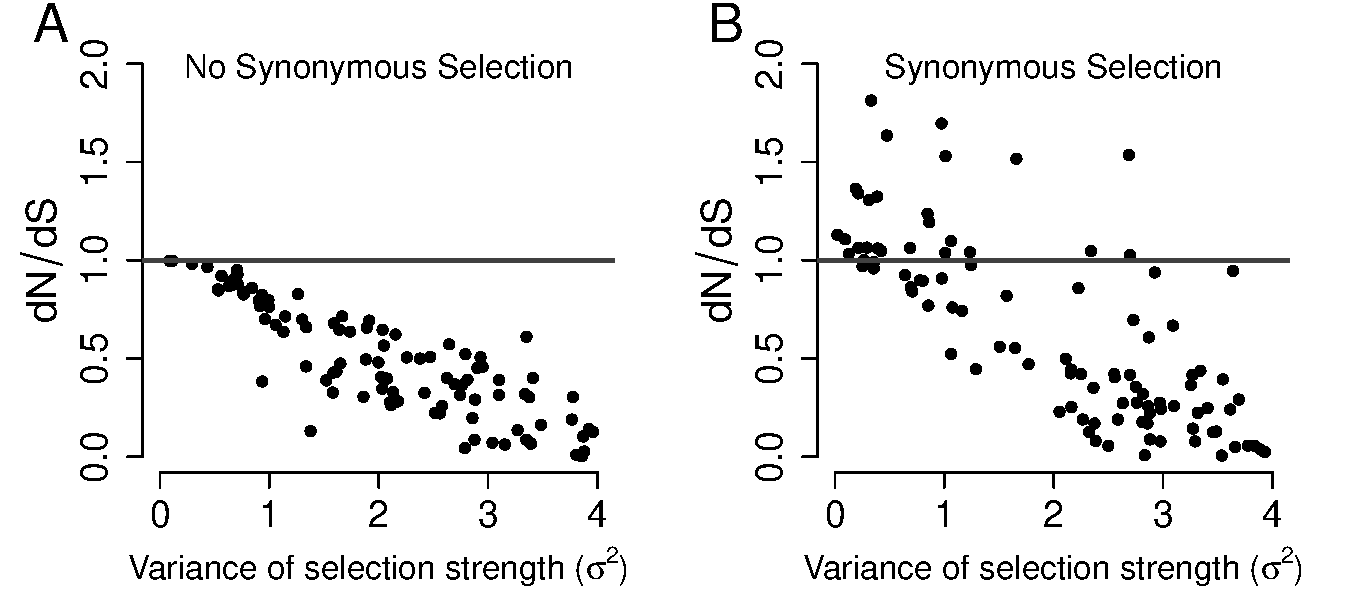
\includegraphics[width=8.7cm]{figures/MainText/dnds_variance.pdf}}
	\caption{\label{dnds_variance} $dN/dS$ decreases in proportion to amino-acid level selection strength. $dN/dS$ is plotted against the $\sigma^2 $ of the simulated distribution of amino-acid scaled selection coefficients. Higher values of $\sigma^2$ indicate larger fitness differences among amino acids, whereas the limiting value of $\sigma^2 = 0$ indicates that all amino acids have the same fitness. (A) Synonymous codons have equal fitness values ($r^2=0.83$). (B) Synonymous codons have different fitness values ($r^2=0.45$). Importantly, (B), but not (A) shows $dN/dS$ values greater than 1, in spite of the steady-state evolutionary process.}
\end{figure}
		
		
\vspace{2cm}
		
\begin{figure}[htbp]
	\centerline{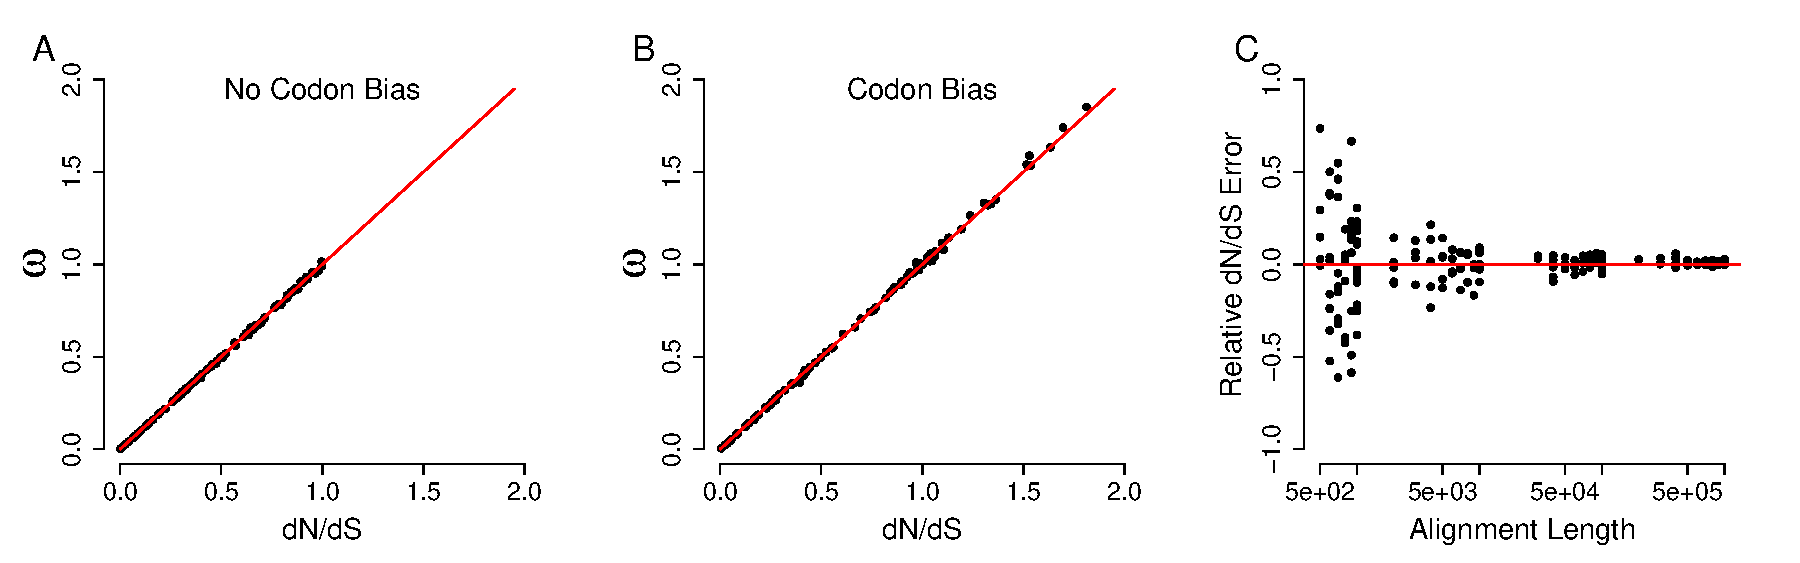
\includegraphics[width=8.7cm]{figures/MainText/regression_convergence.pdf}}
	\caption{\label{reg_conv} Combined modeling approach to assess performance of $dN/dS$ inference frameworks. (A) Protein-coding alignments are simulated in the MutSel modeling framework. $dN/dS$ can then be calculated from scaled selection coefficients as well as through a ML inference framework. Comparing resulting quantities reveals the accuracy in the chosen $dN/dS$ inference framework. (B) Regression between $dN/dS$ values as calculated from scaled selection coefficients and as inferred using the M0 model \cite{GoldmanYang1994,NielsenYang1998,Yangetal2000}. Each point corresponds to a single simulated alignment, and the red line is the $x=y$ line. (C) Convergence of $\omega$ MLEs to the true $dN/dS$ value. The y-axis indicates the relative error of the maximum likelihood $dN/dS$ estimate, and the x-axis indicates the number of positions in the simulated alignment. As the number of positions, and hence the size of the data set, increases, the maximum likelihood estimates converge to the $dN/dS$ values calculated using equations \eqref{eq:pi_i}-\eqref{eq:dS}. The red line is the $y=0$ line, indicating no error.}
\end{figure}
	
\vspace{2cm}
	

\begin{figure}[htbp]
	\centerline{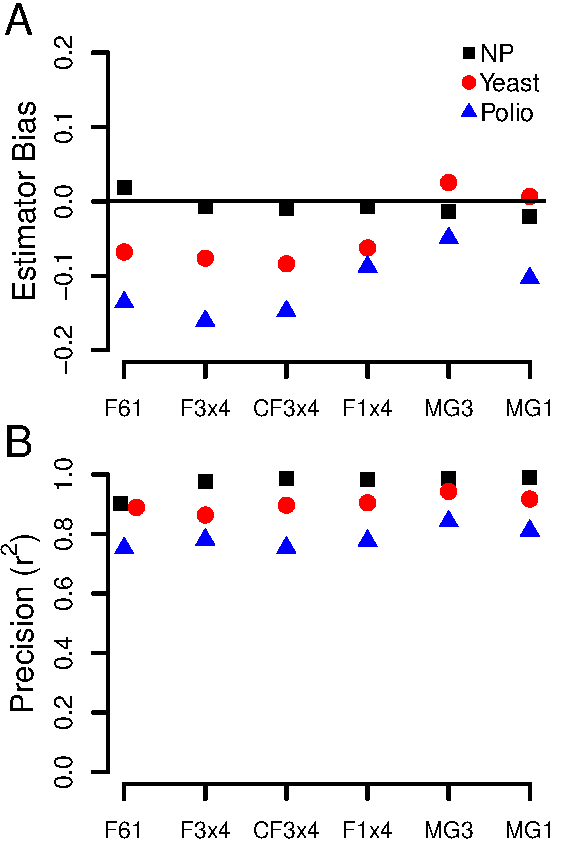
\includegraphics[width=8.7cm]{figures/MainText/nyp_bias_r2.pdf}}
	\caption{\label{nyp_bias_r2} (A) Estimator bias and (B) $r^2$ values between $dN/dS$ and $\omega$ MLEs across model frequency parameterizations, for each set of nucleotide mutation rates. Negative biases indicate $\omega$ estimates that are, on average, lower than $dN/dS$. For all frequency parameterizations, bias generally increases as mutation rates become increasingly asymmetric. Even so, MG-style models tend to yield far less biased $\omega$ estimates than do GY-style models.}	
\end{figure}

\vspace{2cm}


\begin{table}[htbp]
	\caption {\label{tab:dAIC} Mean $\Delta$AIC for datasets simulated with NP, Yeast, or Polio mutation rates.}
	\begin{tabular}{l c c c}
		\hline\noalign{\smallskip}
		\multicolumn{1}{c}{Frequencies} & NP & Yeast & Polio \\
		\noalign{\smallskip}\hline\noalign{\smallskip}
		F61 & 0 & 0 & 0 \\ 
		CF3x4 & -9627.5 & -7951.8 & -7975.9 \\ 
		MG1 & -13325.5 & -10042.0 & -5147.6 \\ 
		F1x4 & -13524.5 & -13658.5 & -15468.3 \\ 
		MG3 & -14401.3 & -12851.6 & -8624.9 \\ 
		F3x4 & -14807.2 & -17385.3 & -19384.6 \\ 
		\noalign{\smallskip}\hline\noalign{\smallskip} 
	\end{tabular}
	Based on AIC scores, the F61 parameterization strongly outperforms all other model parameterizations for all mutation rates, even so the F61 framework yields neither the most accurate nor the most precise parameter estimate. Note that the order of frequency models shown in the table corresponds to the model ranking for NP, and the ranking differs somewhat for yeast and polio datasets. AIC is computed as $AIC = 2(k - \ln(L))$, where $k$ is the number of free parameters of the model, and $\ln(L)$ is the log-likelihood. As codon and/or nucleotide frequency parameters are directly estimated from the data, all models have 3 free parameters ($\omega$, $\kappa$, and a global branch length scaling parameter).
\end{table}

\vspace{2cm}


\begin{figure}[htbp]
	\centerline{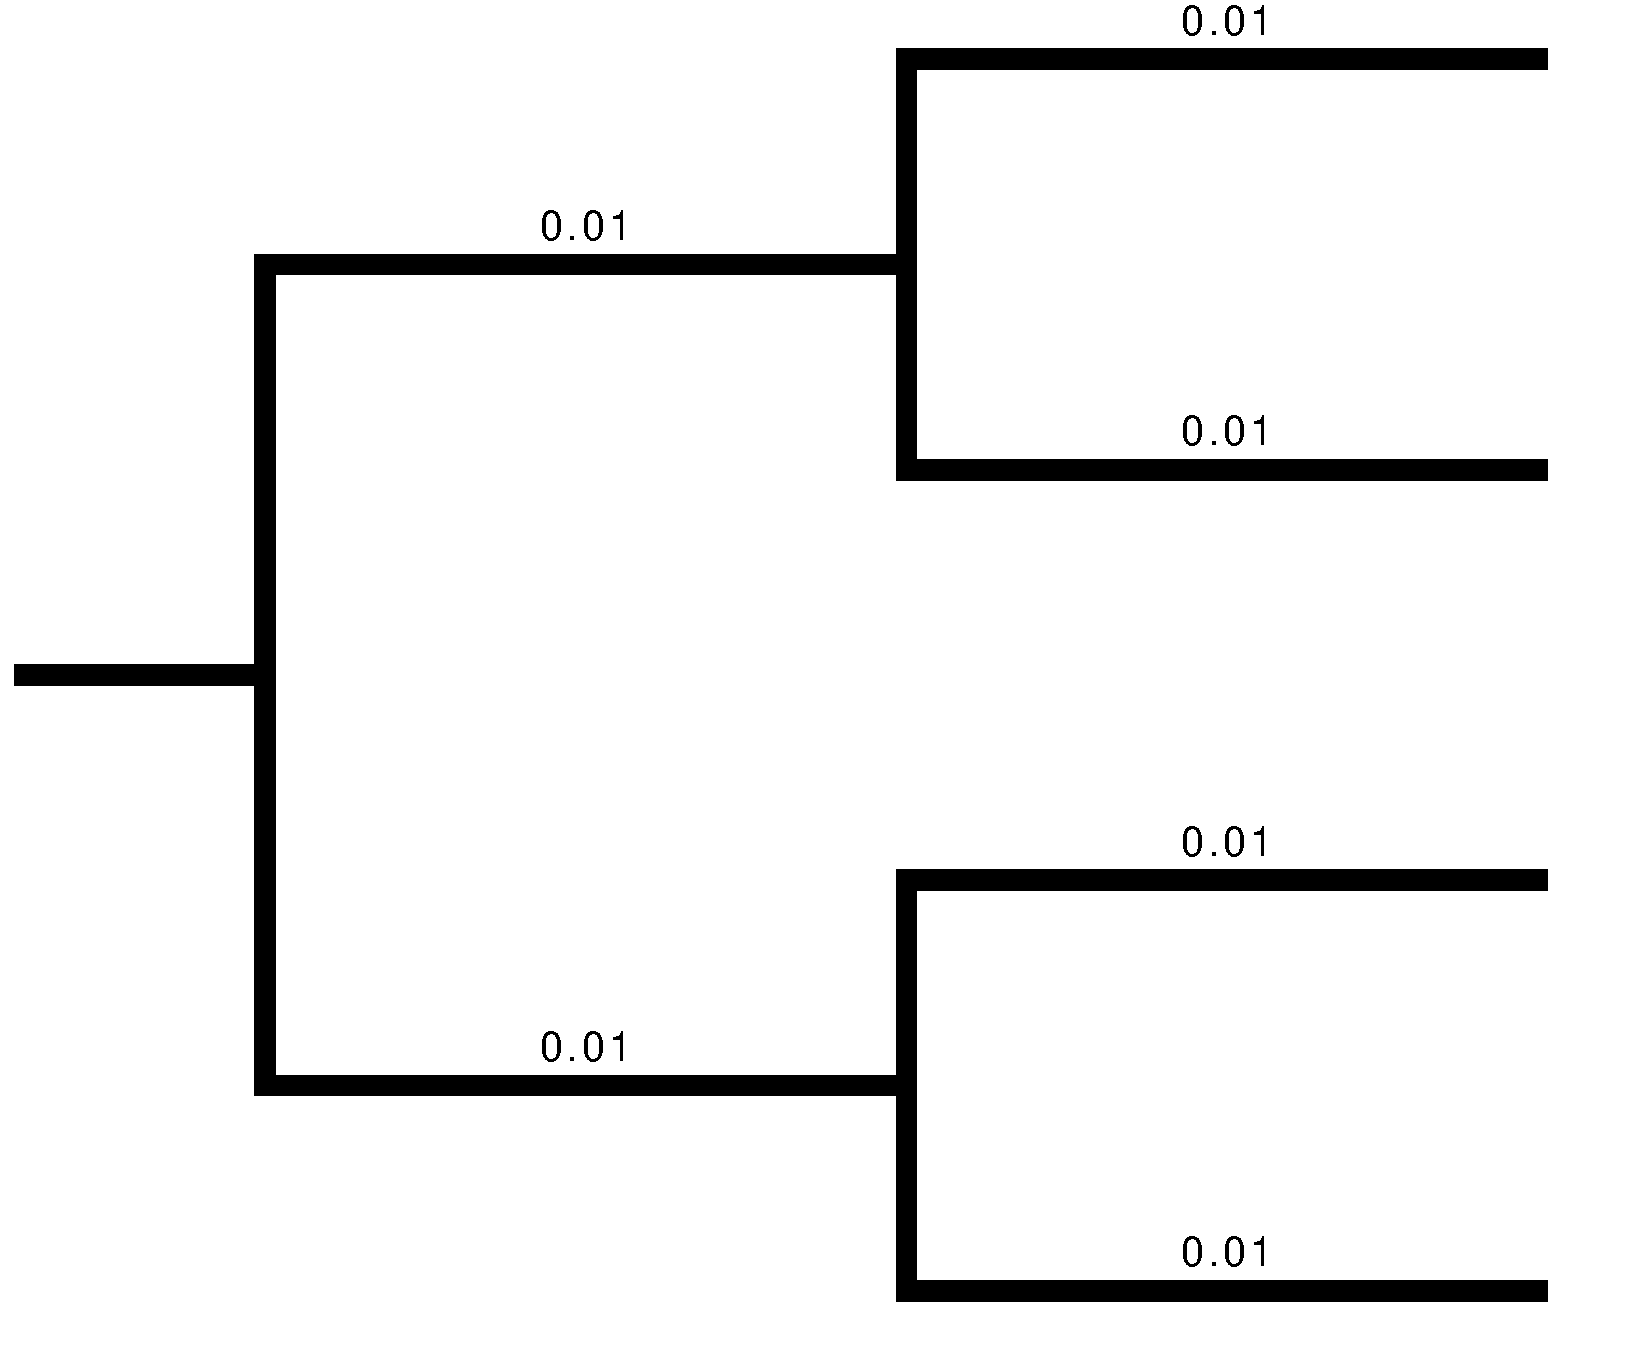
\includegraphics[width=6cm]{figures/MainText/simtree.pdf}}
	\caption{\label{tree} Phylogeny used for all simulated alignments.}	
\end{figure}


\clearpage

	
\section*{Supplementary Information}

\vspace{2cm}

\noindent Table S1. Estimator bias between $\omega$ MLEs and the expected, true $dN/dS$ values, for all mutation rates and model frequency parameterizations examined. Negative bias values indicate that $\omega$ MLEs are, on average, lower than $dN/dS$. All biases are statistically significant, with all $P < 2\times10^{-16}$ except for the estimator bias associated with yeast mutation rates for MG3, where $P = 5.4\times10^{-5}$.
\begin{table}[htbp]
	\begin{tabular}{c c c c c c c}
		\hline\noalign{\smallskip}
		Mutation rate & MG1 & F1x4 & MG3 & CF3x4 & F3x4 & F61 \\
		\hline\noalign{\smallskip}
		NP & -0.014 & -0.02 & -0.007 & -0.009 & -0.007 & 0.019 \\ 
		Yeast & 0.025 & 0.007 & -0.063 & -0.084 & -0.076 & -0.068 \\ 
		Polio & -0.049 & -0.103 & -0.088 & -0.148 & -0.161 & -0.136 \\ 
		\noalign{\smallskip}\hline\noalign{\smallskip}
	\end{tabular}
\end{table}	


\vspace{2cm}

\noindent Table S2. $r^2$ between $\omega$ MLEs and the expected, true $dN/dS$ values, for all mutation rates and model frequency parameterizations examined. All values shown are statistically significant, with all $P < 2\times10^{-16}$ .
\begin{table}[htbp]
	\begin{tabular}{c c c c c c c}
		\hline\noalign{\smallskip}
		Mutation rate & MG1 & F1x4 & MG3 & CF3x4 & F3x4 & F61 \\
		\hline\noalign{\smallskip}
		NP & 0.988 & 0.989 & 0.985 & 0.986 & 0.977 & 0.902 \\ 
		Yeast & 0.943 & 0.917 & 0.905 & 0.897 & 0.864 & 0.889 \\ 
		Polio & 0.842 & 0.811 & 0.777 & 0.754 & 0.781 & 0.752 \\ 
		\noalign{\smallskip}\hline\noalign{\smallskip}
	\end{tabular}
\end{table}	

\newpage

\begin{landscape}
	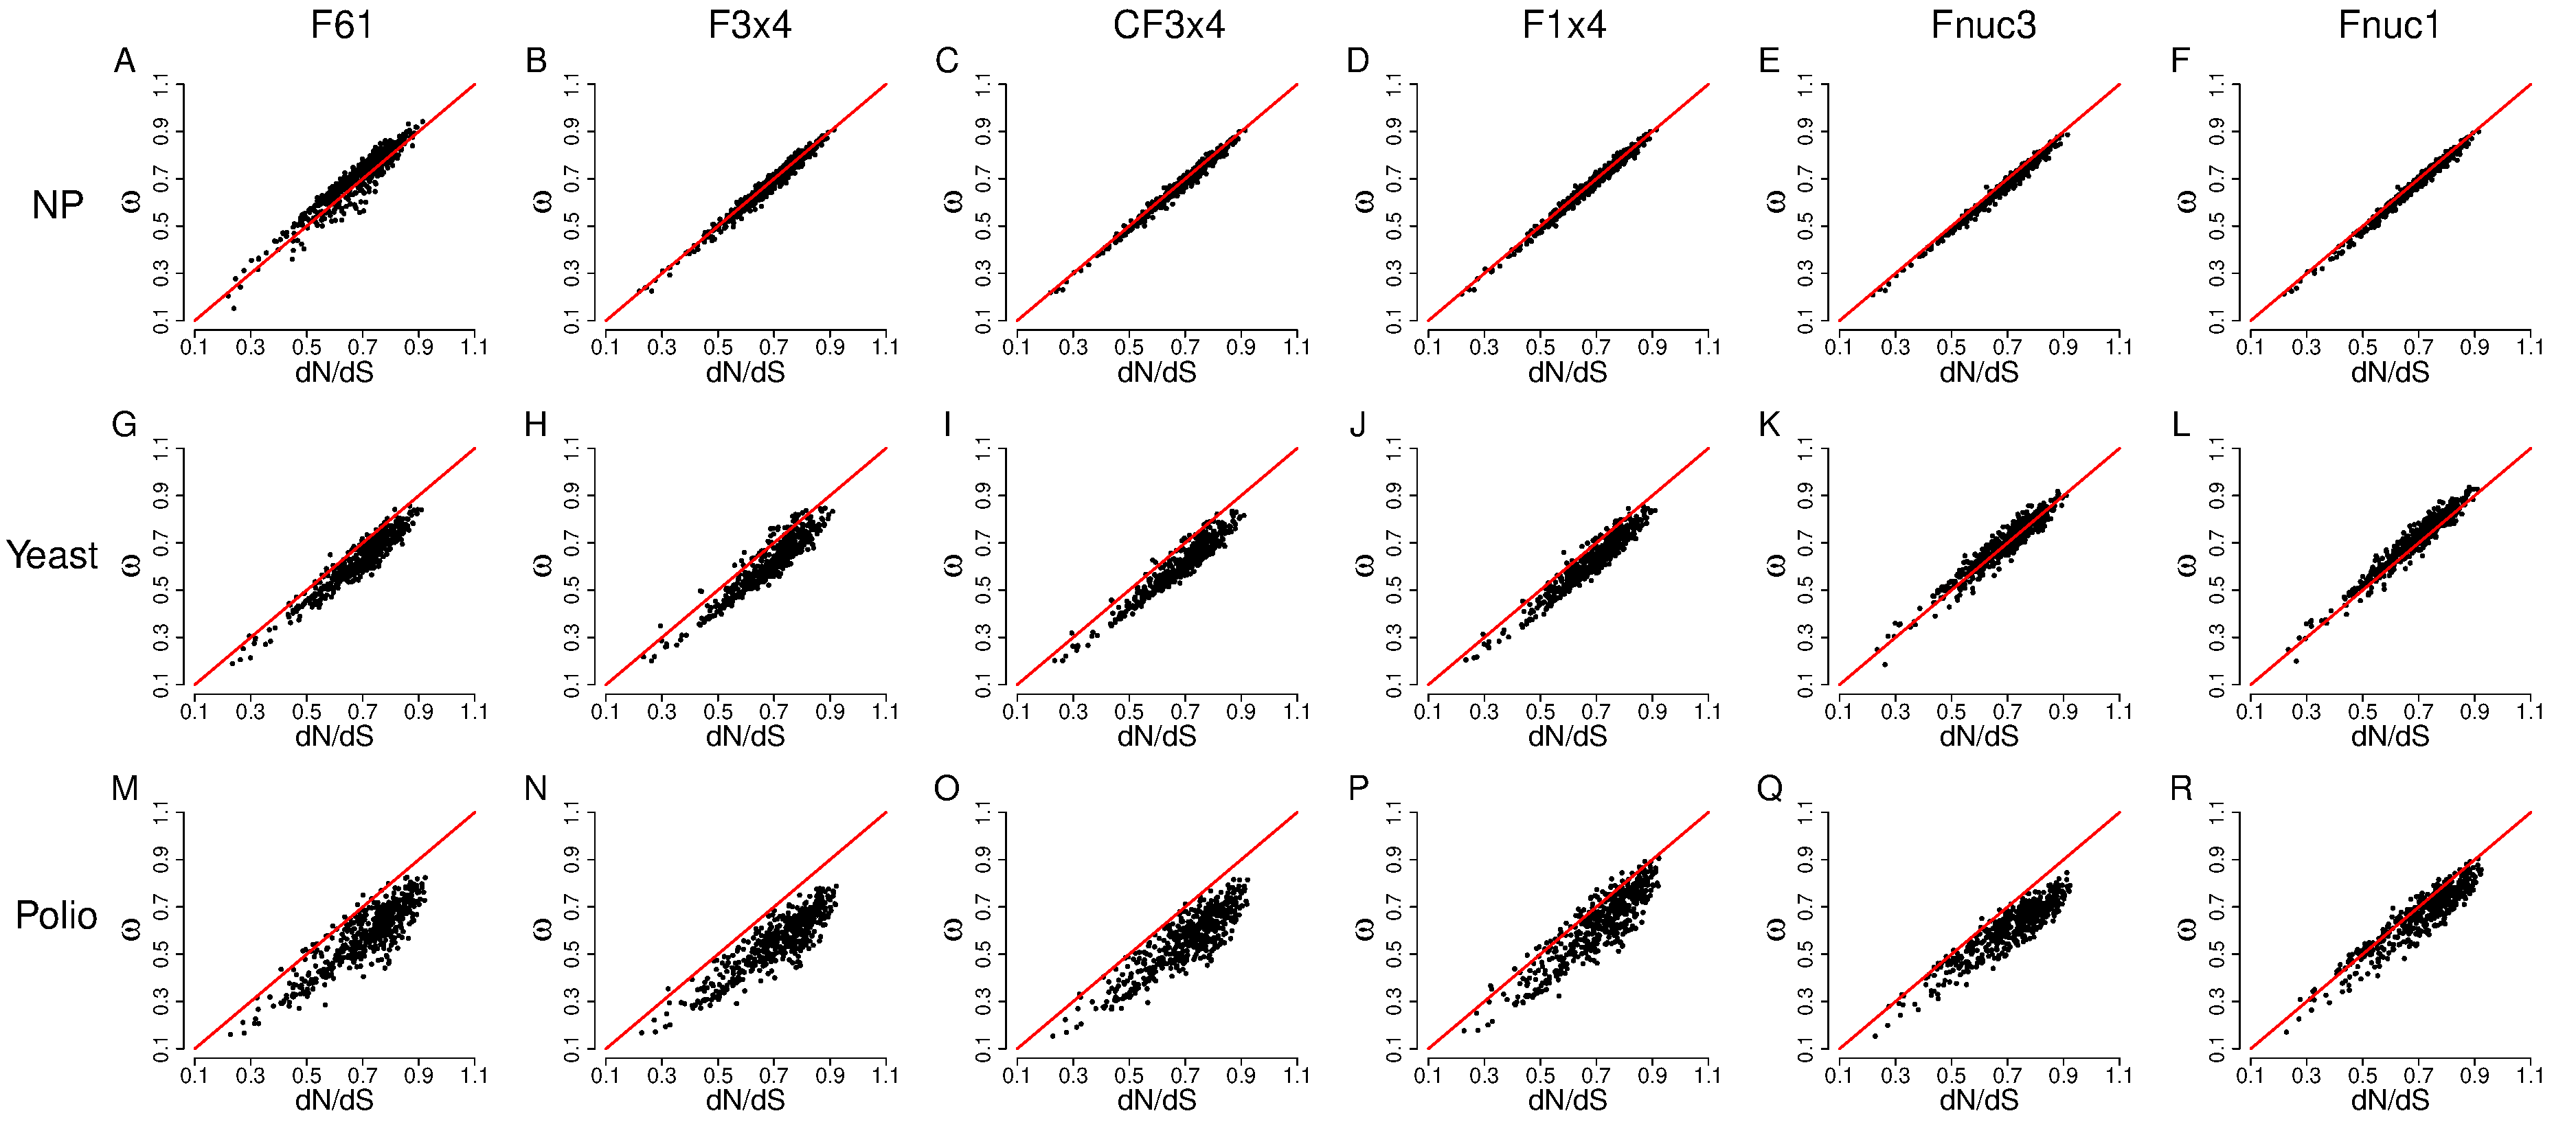
\includegraphics[width=9.5in]{figures/SI/nyp_regression.pdf}
	\vspace{0.5cm}
	
	Figure S1. Regressions for inferred $\omega$ estimates and $dN/dS$ values, as calculated from scaled selection coefficients, for datasets simulated using experimental fitnesses and mutation rates. Each point represents an alignment, and red lines are the $x=y$ line.
\end{landscape}



\end{document}

